\section{Introduction}

% In real-world surveillance and content moderation, anomalous events exhibit a
% ``needle-in-a-haystack'' property---criminal actions may span only seconds within long
% surveillance footage. With the emergence of Vision-Language Models (VLMs) built upon powerful foundations like CLIP~\cite{radford2021learning} and SigLIP~\cite{zhai2023sigmoid}, the field is shifting
% from shallow ``anomaly detection'' (VAD) toward deeper ``anomaly understanding''
% (VAU)~\cite{zhang2024holmes,pi2024vader}, demanding precise event localization, low false
% negative rates, and semantic explanations.

% Despite demonstrating strong zero-shot capabilities on short clips, standard VLMs encounter three critical bottlenecks when deployed on long-form surveillance footage: (1)~\textbf{``Weak Cause--Strong Effect'' misalignment}---the actual
% criminal action (concealed weapon drawing, the ``weak cause'') occupies only seconds, while
% crowd panic (the ``strong effect'') dominates visual change; attention-driven VLMs are drawn
% to the effect, missing the causal onset. (2)~\textbf{Single-pass attention forgetting}---full
% video inference incurs $O(L^2)$ complexity~\cite{vaswani2017attention}, causing subtle early
% events to be overwhelmed by background tokens. (3)~\textbf{Text-mediated information loss}---
% pipelines that convert video to captions (e.g., LAVAD~\cite{zanella2024harnessing}) lose the
% pixel-level micro-evidence needed to detect concealed anomalies.

% To dismantle these barriers, we propose \textbf{Anomaly-Targeted Retrieval (ATR)}, a training-free Visual RAG framework
% that introduces \textbf{Hierarchical Visual Repetition} to the video domain. Inspired by
% RAG~\cite{lewis2020retrieval}, ATR performs \emph{intra-video retrieval} via a
% \emph{VLM-as-a-Retriever} mechanism, achieving temporal grounding while eliminating the need for temporal annotations or parameter fine-tuning. ATR employs a coarse-to-fine dual-stage architecture: \textbf{Scout} globally
% scans for candidate anomalous windows; \textbf{ACE} (Asymmetric Causal Expansion) pads
% windows with aggressive look-back to capture action onset; \textbf{Sniper} jointly processes
% the full global video and the ACE-trimmed focused clip, achieving \textbf{Temporal Zoom-in}
% via heterogeneous dual-view reasoning.

% Video anomaly understanding aims not only to determine whether a long video contains abnormal events but also to identify when they occur and why they should be considered anomalous. 
% Video anomaly understanding aims to determine whether a long video contains abnormal events, provide coarse evidence about where they occur, and explain why they may be considered anomalous. This capability is important for multimedia applications such as surveillance analysis~\cite{sultani2018real}, public safety monitoring, and content moderation. Recent vision-language models (VLMs)~\cite{radford2021learning,zhai2023sigmoid} have shown strong zero-shot performance on short video understanding tasks, suggesting a promising direction toward training-free anomaly understanding. However, their effectiveness remains limited in long-form videos, where abnormal events are often sparse, subtle, and embedded in a lengthy normal context.

Video anomaly understanding aims to determine whether a long video contains abnormal events, retrieve evidence about where they may occur, and explain why they may be considered anomalous. This capability is important for a broad range of multimedia applications, including surveillance analysis, public safety monitoring, and content moderation~\cite{sultani2018real}. Recent vision-language models (VLMs)~\cite{radford2021learning,zhai2023sigmoid} have shown promising zero-shot performance on short video understanding tasks, suggesting a potential path toward training-free anomaly understanding. However, extending this ability to long-form videos remains difficult, since anomalous events are often sparse, subtle, and embedded in lengthy normal context. In this work, candidate timestamps are an intermediate retrieval interface; the final task is video-level judgment and semantic reasoning, not calibrated frame-level boundary prediction.


A central difficulty is selective access to temporal evidence. In surveillance footage, the decisive action may occupy only a few seconds, while the complete scene is still needed to determine whether that action is anomalous. Uniform full-video inference can underemphasize sparse evidence, whereas local-only inference removes the context required for verification. Existing approaches therefore face a tension between \textit{local sensitivity} and \textit{global contextual understanding}. This challenge is further aggravated by the cost of long-context attention~\cite{vaswani2017attention} and by caption-mediated pipelines~\cite{zanella2024harnessing} that may discard subtle visual cues.

% To address these issues, we propose \textbf{A}nomaly-\textbf{T}argeted \textbf{R}etrieval (\textbf{ATR}), a training-free framework for long-form video anomaly understanding. ATR performs coarse-to-fine temporal grounding within a video: it first scans the full video to identify candidate anomalous intervals, then expands the detected interval asymmetrically to recover likely causal context, and finally jointly reasons over the original video and a focused temporal clip. This dual-view design increases the proportion of anomaly-relevant evidence available to the model while preserving global scene context, enabling more reliable anomaly-centric reasoning without temporal annotations or parameter updates.

To address these issues, we formulate anomaly understanding as content-relevant intra-video retrieval followed by global--local verification. Based on this formulation, we propose \textbf{A}nomaly-\textbf{T}argeted \textbf{R}etrieval (\textbf{ATR}), a training-free two-call framework. Scout first scans the complete video and proposes candidate intervals. Sniper then receives two visual inputs together: the same complete original video and a focused clip cut from it. The complete video is never replaced by a crop; the local clip provides a denser second view while the full video preserves scene and temporal context. A fixed temporal padding rule supplies surrounding context before clip extraction. The framework requires neither temporal annotations nor parameter updates.

\begin{figure*}[t]
  \centering
  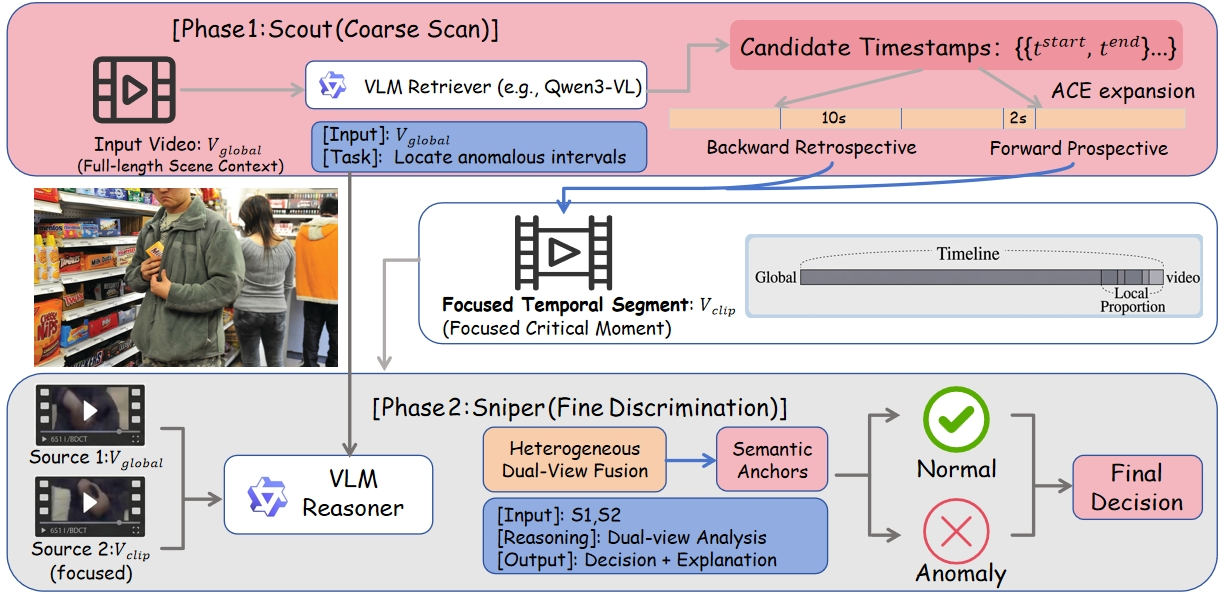
\includegraphics[width=0.915\linewidth]{figures/fig_framework.png}
  \caption{Overview of the ATR framework. The Scout module performs global scanning to
  identify candidate anomalous windows. A fixed temporal padding rule retains nearby context before clip extraction. The Sniper
  module performs heterogeneous dual-view reasoning over the full global video and the
  focused temporal segment simultaneously.}
  \label{fig:framework}
\end{figure*}
Extensive experiments on UCF-Crime show that ATR substantially reduces missed anomalies for lightweight VLMs. Strict matched controls separate content selection from an extra model call, additional tokens, and arbitrary clips, while evidence-removal tests verify that Sniper uses the retrieved view. An 8B ATR configuration also outperforms a substantially larger 32B global-only baseline at about one tenth of its GPU-hour cost. Additional experiments across model families and an audio-visual benchmark characterize how the operating point transfers beyond the primary setting.

The main contributions can be summarized as follows:

% \begin{enumerate}
%   % \item \textbf{Hierarchical Visual Repetition and the ATR Framework}: We introduce \textbf{Hierarchical Visual Repetition}, enabling efficient heterogeneous dual-view reasoning. With only $\sim$5\% additional tokens, ATR reduces the 4B model's FNR by 56.8\% relative to baseline and achieves 85.17\% accuracy. The 8B model reaches 85.52\%, surpassing the 32B baseline (83.45\%), proving that intelligent retrieval can substitute for model scale.

%   % \item \textbf{ACE: Asymmetric Causal Expansion}: A targeted temporal calibration mechanism addressing ``weak cause--strong effect'' asymmetry. Validated as a reliable positive calibrator, ACE consistently improves FNR and F1 without degrading accuracy, scaling with Scout localization precision.

%   % \item \textbf{Over-Alignment Phenomenon}: We identify that excessive safety alignment in 32B models compromises sensitivity. ATR yields negative gains on 32B but positive gains on 4B/8B, attributed to 32B's high Scout failure rate (62.4\%) and safety alignment interference~\cite{ouyang2022training,askell2021general}.

%   \item We propose ATR, a training-free framework that formulates long-form video anomaly understanding as an intra-video coarse-to-fine retrieval problem. ATR combines global scanning, asymmetric causal expansion to recover pre-anomaly context, and dual-view reasoning---enabling anomaly understanding without temporal annotations or parameter updates.

%   \item Through extensive experiments on UCF-Crime, XD-Violence, and multiple VLM backbones (Qwen3-VL, Qwen3.5-VL, Qwen2.5-Omni), we show that ATR consistently benefits lightweight models while revealing a dual-stage over-alignment phenomenon in larger models. These findings delineate empirical applicability boundaries for retrieval-augmented video understanding.
% \end{enumerate}

\begin{itemize}
    \item We propose \textbf{ATR}, a training-free selective re-reading framework that jointly presents the complete video and a content-relevant local view, preserving global context without temporal annotations or parameter updates.
    
    \item We provide a \textbf{mechanism-focused evaluation} using Second Global, duration-matched Random and Uniform clips, and Source~2 removal. These controls distinguish extra computation, token volume, content selection, and actual evidence use.
    
    \item We establish practical \textbf{accuracy--efficiency operating points}: ATR enables lightweight VLMs to reduce missed anomalies and outperform a 32B global-only baseline at roughly 10\% of its GPU-hour cost, with FNR/FPR and cross-backbone results reported jointly.
\end{itemize}
